\documentclass{standalone}
\usepackage{tikz}
\begin{document}
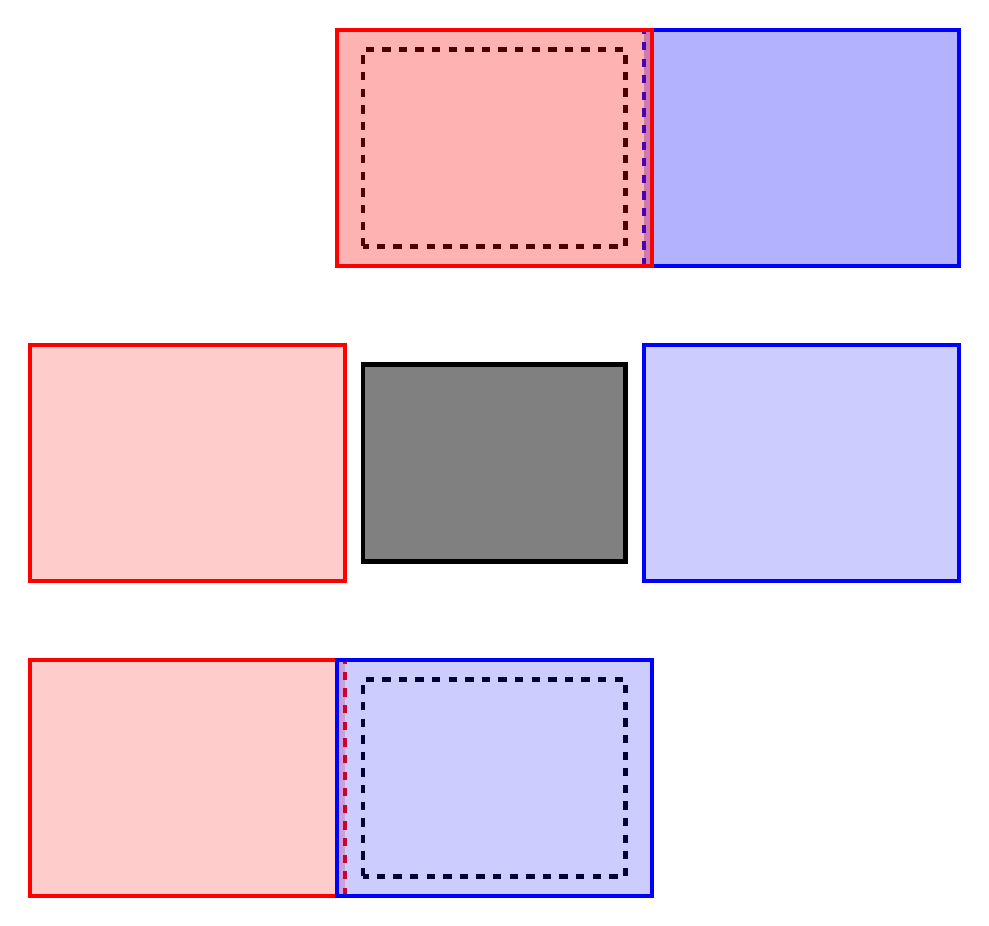
\begin{tikzpicture}

\def\sceneAy{0}
\def\sceneBy{4}
\def\sceneBy{8}
\def\sceneH{4}

\def\planeW{4}
\def\planeH{3}
\def\planeSep{-0.1}
\def\backW{3.333}
\def\backH{2.5}
\def\backX{0.333}
\def\backY{0.25}
\def\clrfirst{red}
\def\clrsecond{blue}
\def\clrback{black}

\begin{scope}[ultra thick]
		\draw [\clrsecond,dashed] (\planeW+\planeSep, 0) -- ++(0,\planeH);
		\draw [\clrsecond,fill,fill opacity=0.3]        (\planeW+\planeSep,\planeH)
		      -- ++(\planeW,0) -- ++(0,-\planeH) -- ++(-\planeW,0);
		\draw [\clrback,dashed] (\backX,\backY) rectangle ++(\backW, \backH);
		\draw [\clrfirst,fill=\clrfirst,fill opacity=0.3] (0,0) rectangle ++(\planeW,\planeH);

	\begin{scope}[yshift=-{\sceneH}cm]
		\draw [\clrfirst,fill,fill opacity=0.2] (-\planeW-\planeSep,0) rectangle ++(\planeW,\planeH);
		\draw [\clrback,fill=gray] (\backX,\backY) rectangle ++(\backW, \backH);
		\draw [\clrsecond,fill,fill opacity=0.2] (\planeW+\planeSep, 0) rectangle ++(\planeW, \planeH);
	\end{scope}

	\begin{scope}[yshift=-{2*\sceneH}cm]
		%\draw [\clrfirst] (-\planeW-\planeSep,0) rectangle ++(\planeW,\planeH);
		\draw [\clrfirst,dashed] (-\planeSep, 0) -- ++(0,\planeH);
		\draw [\clrfirst,fill,fill opacity=0.2]        (-\planeSep,\planeH)
		      -- ++(-\planeW,0) -- ++(0,-\planeH) -- ++(\planeW,0);
		\draw [\clrback,dashed] (\backX,\backY) rectangle ++(\backW, \backH);
		\draw [\clrsecond,fill,fill opacity=0.2] (0, 0) rectangle ++(\planeW, \planeH);
	\end{scope}
\end{scope}

\end{tikzpicture}
\end{document}
